\section{Physiological Abstraction rules}
\label{abstractionRules} 
In this section, domain-specific abstraction rules are developed that can introduce new behaviors to a given heart model or set of models. 
These new behaviors are physiologically meaningful and might be manifested by a heart condition not explicitly modeled in the initial set of models.
The physician (or domain expert) remains the ultimate arbiter of what is physiologically meaningful.
This is a peculiarity of environment modeling, borne out of the fact that the initial set of models is necessarily incomplete, and does not represent all valid behaviors.
We then show how the application of these domain-specific rules can be automated, thus obviating the need for domain expertise.

Recall that heart conditions are modeled as finite directed labeled graphs as introduced in Def.~\ref{def:labeledGraph}.
%Let $\Gc$ be the set of labeled graphs, and $2^\Gc$ be the power set of $\Gc$.
%An abstraction rule is a function $2^\Gc \rightarrow \Gc$.
Rules operate on a graph only if it has the appropriate structure for that rule, and if its parameters meet certain rule-specific conditions (if any).
Due to space limits only a subset of the abstraction rules are introduced. 
The full set is in the technical report \cite{regar_tech}.

% such that 
%\begin{enumerate}
%	\item $|V(R(G))| \leq |V(G)|$
%	\item $|E(R(G))| \leq |E(G)|$
%	\item The model $R(G)$ is an over-approximation of $G$ in the sense of Section \ref{overapx}.
%\end{enumerate}
%Some rules modify only a portion of the graph $G$.
%We introduce some notation: given a graph $G$ and an element $x \in V(G) \cup E(G)$ of $G$, we write $A_x$ for the automaton labeling that element.
%We write $\Ac(G)$ for the set of automata of a graph: $\Ac(G) = \{A_x : x \in V(G) \cup E(G)\}$.
%The set of parameters of the automaton is written $\Pc(A_x) = \{\theta_1^x,\theta_2^x,\ldots\}$. 
%Recall that a parameter $\theta$ has both a minimum $\theta_{min}$ (which is used in the guard definitions of the automaton) and a maximum $\theta_{max}$ (which is used in the invariant definition of the automaton).

%\subsection{Rule 1: Convert Reentry Circuits to Activation Nodes}
Within the conduction network of the heart, there can be multiple pathways between two locations, forming conduction loops. If the timing parameters of the tissue along the loop satisfy certain property, there can be scenarios in which an depolarization wave circling the circuit. The circuits are referred to as \emph{Reentry Circuits}. Since the time interval for an activation wave to circle a reentry circuit is usually less than the intrinsic heart cycle length, the heart rate will be "`hijacked"' by the reentry circuit once the cycling is triggered, causing tachycardia. Reentry is the most common mechanism for tachycardia which can be modeled by our heart models \cite{vhm_embc10}. 

The effect of reentry tachycardia is that activation signals coming out of the circuit with cycle length equals to the sum of conduction delays of the conduction paths forming the circuit. It is therefore reasonable to model a reentry circuit as a self-activation node with the self-activation range equal to the sum of conduction delays. For more complex structures with multiple circuits, the self-activation range will be the minimum of the shortest circuit to the maximum of the longest circuit. The detailed rule description and implementation can be found in %\cite{regar_tech}.
%\begin{figure}[!h]
%\centering
%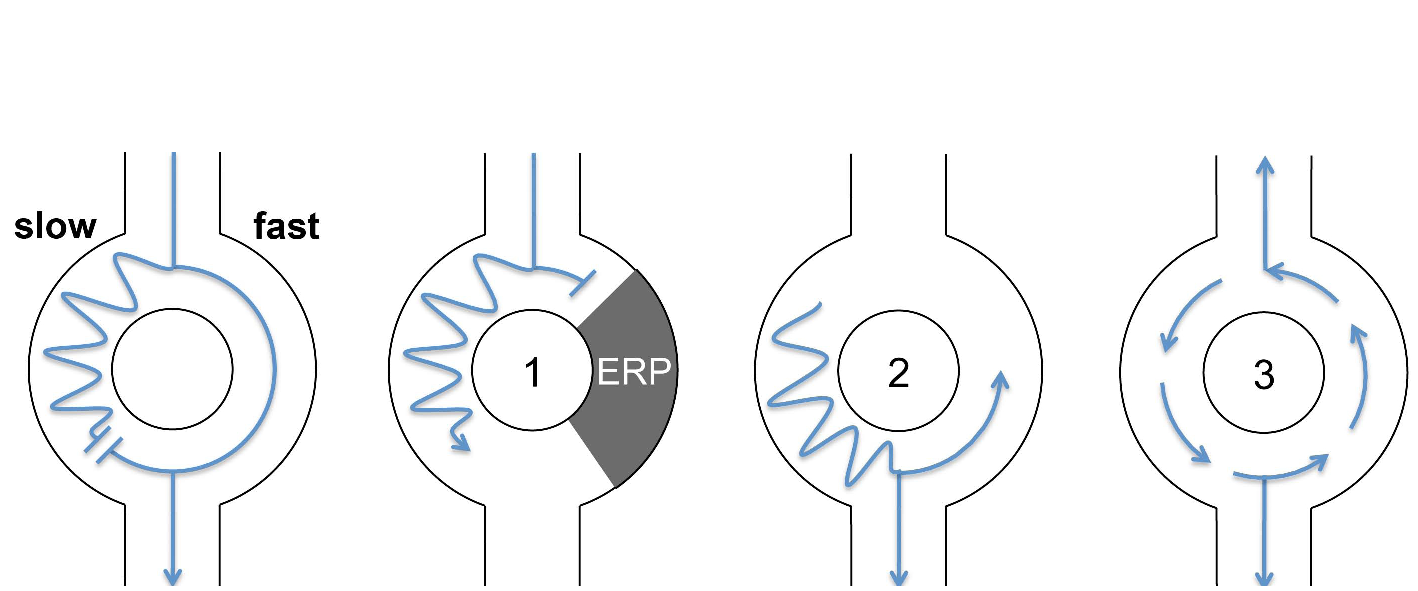
\includegraphics[width=0.6\textwidth]{figs/reentry.pdf}
%%\vspace{-5pt}
%\caption{\small Reentry Circuit}
%%\vspace{-15pt}
%\label{fig:reentry}
%\end{figure}

%\subsubsection{Rule 2: Remove Irrelevant Structures}
The network of node and path automata can be viewed as a graph,with nodes as vertices, paths as edges with conduction delay as weight. After the loops within the topology are removed, the topology of the heart model is in form of tree. Within the network there are certain nodes that are more important in terms of model behaviors, we denote them as \emph{Nodes of Interests}, which include:
\begin{itemize}
\item Nodes with self-activations
\item Nodes which interact with the pacemaker
\end{itemize}
Graph algorithm can be performed on the heart model to identify the core structure. Shortest paths can be calculated among nodes of interests. All the nodes and paths along the shortest paths are regarded as core structure. All the other nodes and paths can be then removed without affecting the behaviors of the model. 
%\todo[inline]{Not true. Teh behavior is affected. Because this is a formal methods conference, so behavior and so on mean very specific things.}
\subsubsection{Rule 3: Removing Unnecessary Non-self-activation Nodes}
The effect of non-self-activation nodes is blocking electrical events with interval shorter than its ERP period. If the self-activation nodes at both ends of a core path have self-activation interval longer than the maximum ERP period of nodes along the core path, the nodes can be removed.

For a core path from a self-activation node $N_1$ to another core node $N_2$, for any structure $P_1-N_n-P_2$ which $N_n$ is a non-self-activation node, if $N_n.ERP_{max}<min(N_1.Rest_{min},N_2.Rest_{min})$, replace $P_1-N_n-P_2$ with $P_3$ so that:
$$P_3.cond_{min}=P_1.cond_{min}+P_2.cond_{min}$$
$$P_3.cond_{max}=P_1.cond_{max}+P_2.cond_{max}$$

\subsection{Rule R4: Merge Parameter Ranges}
\textbf{Physiological intuition}. 
Timing periods of heart tissue, like Rest and ERP, are modeled as locations in the node and path automata. 
The minimum and maximum time an automaton can stay in a location is governed by the parameters in the guards and invariants. 
By expanding these periods, we introduce new behavior where a heart may stay in Rest for longer, or (self-)activate a node faster, etc.
\\
\textbf{(Sub)graph(s) to which it applies}.
This rule applies to a set of graphs $G_i$ with the same structure (i.e., they are pairwise isomorphic) but possibly with different parameters: $R(G_1,\ldots,G_n) = G'$.
See Fig.~\ref{fig:HM_abs}.\\
\textbf{Applicability conditions}.
None.\\
\textbf{Output (sub)graph}.
$G'$ has the same structure as the $G_i$.
Thus there's an isomorphism $f$ between every $G_i$ and $G'$.
Given an element $x$ of $G'$, $f^{-1}(x') = \{x_1,\dots,x_n\}$ are used to represent the set of elements that map to it via $f$.\\
\textbf{Effect on parameters}
%Recall Def.~\ref{def:labeledGraph}
For every automaton $A_{x'} \in \Ac(G')$, and every parameter $\theta^{x'}$ of $A_{x'}$, 
$\theta_{min}^{x'} = \min(\theta^x_{min})_{x \in f^{-1}(x') }$ and 
$\theta_{max}^{x'} = \max(\theta^x_{max})_{x \in f^{-1}(x') }$
\textbf{Proof of abstraction} A detailed proof can be found in \cite{regar_tech}.

%\subsection{Rule 5: Merge Self-activation Nodes with Interaction Nodes}
%\todo[inline]{not clear}
The effect of self-activation nodes on the interaction of the pacemaker is triggering sensing events within certain delay. In this rule we merge all the self-activation nodes to their neariest interaction nodes. If there exists multiple self-activation nodes merging to the same interaction node, the parameters of the new model are determined following Rule 3.


\subsection{Rule R6: Replace Blocking With Non-deterministic Conduction}
\textbf{Physiological intuition}. 
%\todo[inline]{in modeling section mention self-activating and passive nodes}
%If a node automaton is in its \textsf{ERP} state, a \textsf{Act\_node} event is "blocked" and will not trigger corresponding path conduction. If we add non-deterministic transitions to the path automata such that a \textsf{Act\_path} event do not trigger state transitions to \textsf{ante} or \textsf{retro} (\figref{rule5}), the blocking behavior of the node is covered. We can then merge the \textsf{ERP} state with the \text{Rest} state in the node automata, and all passive nodes can be removed. An application of Rule 6 is shown in \figref{abs_exam}.\\
Consider the structure $N_1 P_1 N_2 P_2 N_3$ with three nodes and two paths, where $N_2$ is a passive node (i.e. not self-activating).
If $N_2$ blocks an activation signal from $N_1$ to $N_3$, this is equivalent to the paths $P_1$ or $P_2$ not conducting.
In this rule, the structure $P_1 N_2 P_2$ is replaced by a path $P$ whose automaton can take a self loop when it receives an activation signal, thus effectively stopping the conduction. 
This is shown in Fig.~\ref{fig:rule5}: the extra transitions are marked {\quattrofont Act\_path\_1?} and {\quattrofont Act\_path\_2?}.
Because the blocking effect of nodes is now incorporated into the paths, the node automata of self-activating nodes can be modified to the one shown in Fig.~\ref{fig:rule5}, which doesn't have the (now useless) ERP period.
\\
\textbf{Subgraph to which it applies}.
Line graphs with 3 vertices $N_1 P_1 N_2 P_2 N_3$, and self-activating nodes.\\
\textbf{Applicability conditions}.
$N_2$ is a passive node.\\
\textbf{Output subgraph}.
$N'_1 P' N'_3$
A path $P'$ whose path automaton is as shown in Fig.~\ref{fig:rule5}.b.
The self-activating nodes $N$ are replaced by nodes $N'$ with automata shown in Fig.~\ref{fig:rule5}.a.\\
\textbf{Effect on parameters}
For the new path, $P.cond_{min}=P_1.cond_{min}+P_2.cond_{min}$ and 
$P.cond_{max}=P_1.cond_{max}+P_2.cond_{max}$
For the new nodes, $N'.Trest_{min}=N.TERP_{min}+N.Trest_{min}$ and 
$N'.Trest_{max}=N.TERP_{max}+N.Trest_{max}$.\\
\textbf{Proof of abstraction} Timed simulation relationship between $N_1 P_1 N_2 P_2 N_3$ and $N'_1 P' N'_3$ is proved in \cite{sttt13}.

\begin{figure}[!t]
	\centering
	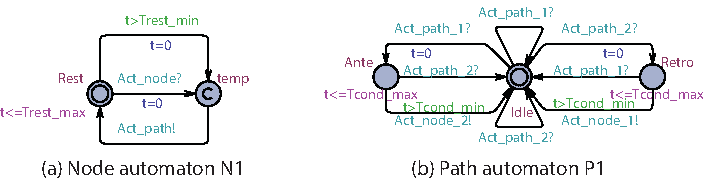
\includegraphics[width=0.9\textwidth]{figs/rule5.pdf}
	%\vspace{-5pt}
	\caption{\small Node and Path Automata after application of Rule 6 and 7}
	%\vspace{-15pt}
	\label{fig:rule5}
\end{figure}

\subsection{Rule R7: Replace Conductions With Self-activation}
\textbf{Physiological intuition}. 
The effect of a conduction path is to conduct electrical activity generated by a self-activation node to other nodes. 
If all self-activation nodes are allowed to activate at any time by setting their Rest period to $[0,+\infty]$, all the conduction paths can be removed, while preserving the original behavior (where the Rest period was constrained to a finite interval).
An application of Rule 7 is shown in \figref{abs_exam}.
\textbf{Subgraph to which it applies}.
The entire graph $G$.\\
\textbf{Applicability conditions}.
This rule can only be applied after Rule 5 has been applied.\\
\textbf{Output subraph}.
All edges are deleted: $G' = (V(G), \emptyset)$. The node automata are replaced with the one shown in \figref{rule5}.c.\\
\textbf{Effect on parameters}
For every node automaton $N$ in $G'$, the node automata are $N.Trest_{min}=0,N.Trest_{max} = +\infty$.\\
\textbf{Proof of abstraction} Detailed proof can be found in \cite{regar_tech}.

%\begin{figure}[!h]
%	\centering
%	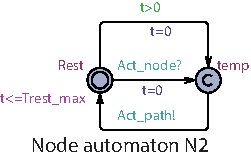
\includegraphics[width=0.3\textwidth]{figs/rule6.pdf}
%	%\vspace{-5pt}
%	\caption{\small Node automata after application of Rule 7}
%	%\vspace{-15pt}
%	\label{fig:rule6}
%\end{figure}

%\subsection{Automatic rule application}
\label{automatedApplication}

Because we start from a set of initial models, and have a set of abstraction rules that can be applied to any given model, we have a choice of which rules to apply to which models, and the order in which to apply them.
E.g. consider the labeled graph of Fig.???, to which both rules R6 and R7 are applicable.
Depending on which rule is applied first, we end up with different abstract models.
In this section we propose a measure of abstractness, and sketch how an optimal order of application can be found as the solution of a Mixed-Integer Nonlinear Program (MINLP).
Details can be found in the technical report. 

First, we observe that when a rule is applied to a labeled graph $G=(V,E,A)$, it either decreases the number of vertices, or the number of edges, or it enlarges the invariant and/or guard sets of some of the automata (by manipulating the parameters as done, e.g., by Rule 4).
We define a measure of the abstraction power $\alpha(R)$ of a rule $R$ to be
\[\alpha(R) = |V(G)| - |V(R(G))| + |E(G)| - |E(R(G))| + \sum_{x \in \Ec(G)\cap \Ec(R(G))}|\theta^x - R(\theta^x)|\] 
Intuitively, a rule $R$ is more abstract than rule $R'$ if it removes more elements of enlarges the parameter ranges more.

Rule application must respect the following constraints, all of which can be encoded as the constraints of a MINLP:
\begin{enumerate}
	\item Only one rule can be applied at a time.
	\item A rule can only be applied to a (sub)graph with a given structure, and whose parameters respect certain conditions.
	\item When a rule is applied to a subgraph, it may disable future rule applications to this subgraph, either because a) it changed the subgraph's structure, or b) it updated the subgraphs's parameters.
\end{enumerate}
We define binary variables $a_{isj}$ such that $a_{isj} = 1$ iff at the $j^{th}$ time step, we apply rule $R_i$ to subgraph $K_s \subset G$.
The first constraint, for example, can be encoded as
\[\forall j=1,\ldots, N, \sum_{i,s}a_{isj} \leq 1\]

Proceeding in this manner, we formulate a MINLP whose solution gives an optimal order of rule application, in the sense of maximizing the abstractness of the final model.
Then model-checking can be performed on this most abstract model, which, by construction, covers the most behavior.

\subsection{Heart Model Abstraction Tree}
A list of heart models corresponding to common heart conditions are first developed. The list can be expanded as new heart conditions are discovered.
By systematically applying rules in this section an abstraction tree $HM\_tree$ for the heart is created (\figref{HM_abs}). 
%Note that applying rules in different order results different abstraction tree. 
%The order used to obtain $HM\_tree$ is based on the domain knowledge that certain heart conditions may have similar behaviors and similar inputs to the pacemaker. 
%This systematic grouping maintains the physiological-relevance of the heart model even at higher abstraction levels, and reduce the necessity to resolve ambiguities at lower abstraction levels when model checking certain requirements.
\begin{figure}[!t]
	\centering
	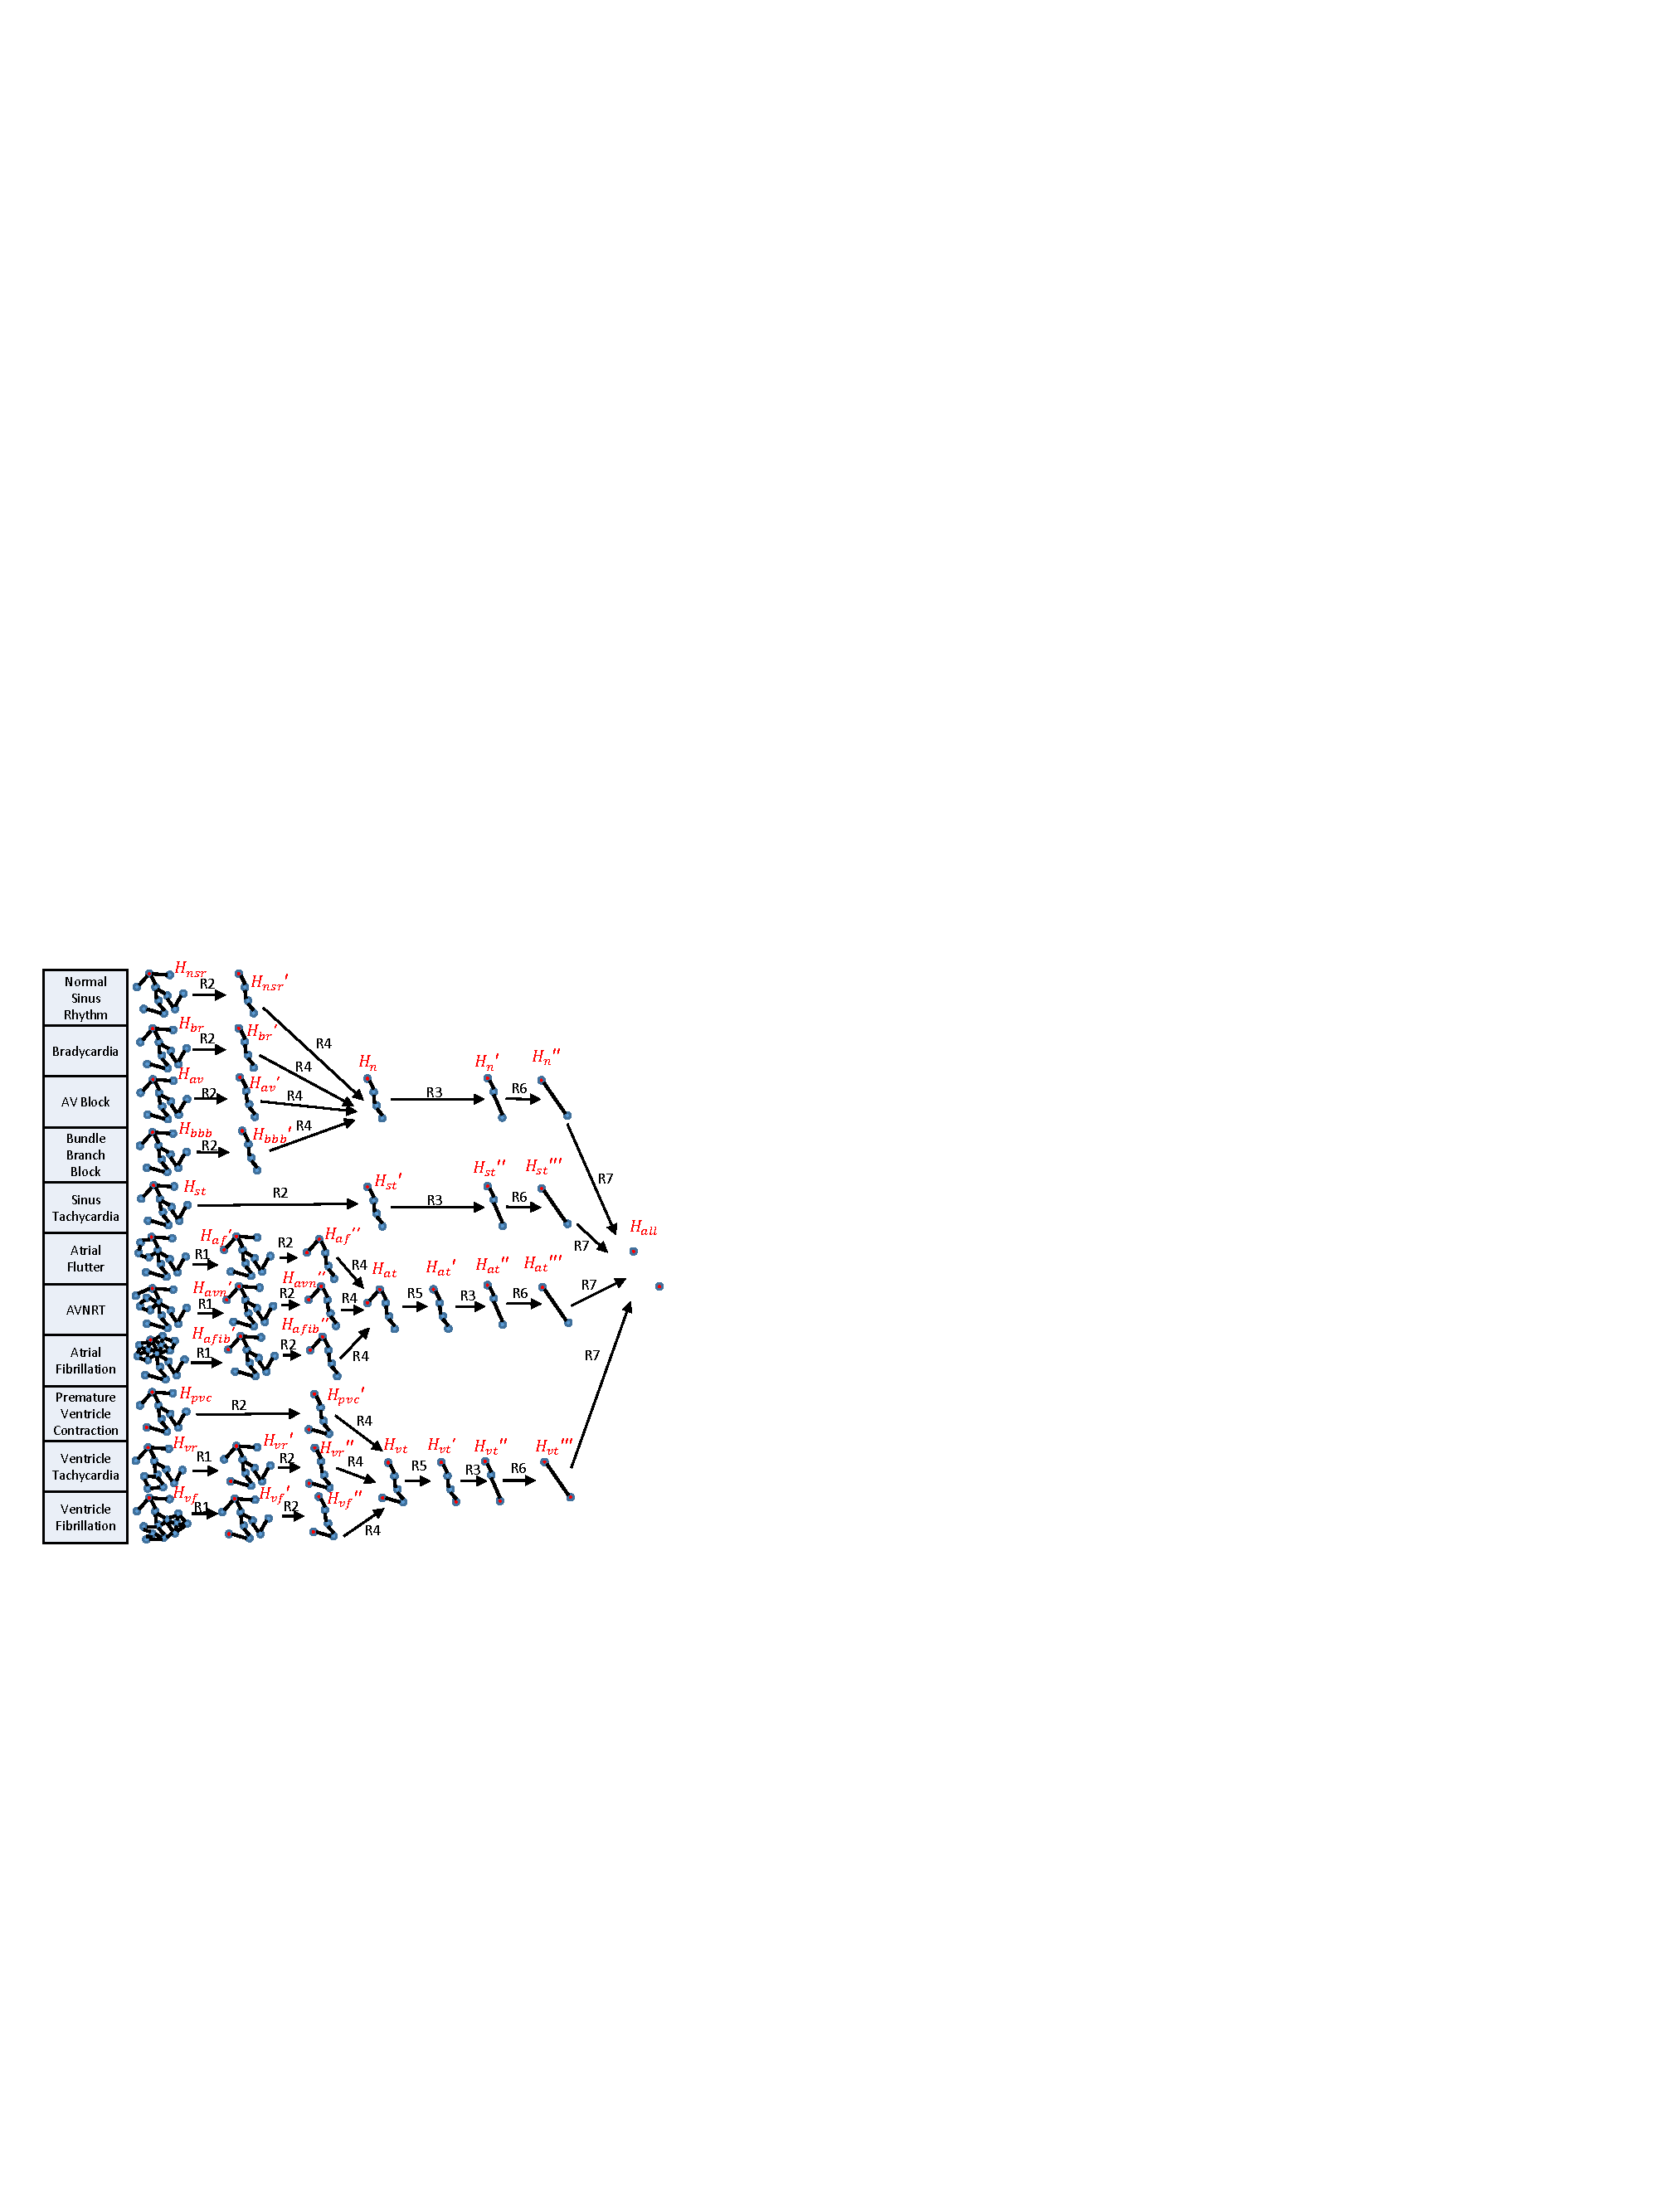
\includegraphics[width=0.9\textwidth]{figs/abs.pdf}
	%\vspace{-5pt}
	\caption{\small Heart Model Abstraction Tree}
	%\vspace{-15pt}
	\label{fig:HM_abs}
\end{figure}


%\subsection{Rule Application Example}
%In this section we demonstrate 
%\todo[inline]{I don't understand what this is...}
%$$NA\_self=\{SA\_self,AVNRT\_self,AF\_self,PAC\_self\}$$
%$$NV\_self=\{PVC\_self,VF\_self,VT\_self\}$$
%$$(NA,AV')\_cond=\{(SA,AV)\_cond\}$$
%$$(AV',NV)\_cond=\{(AV,RBB)\_cond,RBB-RVA\_cond\}$$
%Apply Rule 6:
%$$NA'\_self=\{NA\_self\}$$
%$$NV'\_self=\{NV\_self\}$$
%$$(NA',NV')\_cond=\{AV'\_block,(NA,AV')\_cond,(AV',NV)\_cond\}$$
%Apply Rule 7:
%$$NA''\_self=\{NA'\_self,(NA',NV')\_cond\}$$
%$$NV''\_self=\{NV'\_self,(NA',NV')\_cond\}$$
%\begin{figure}[!t]
%\centering
%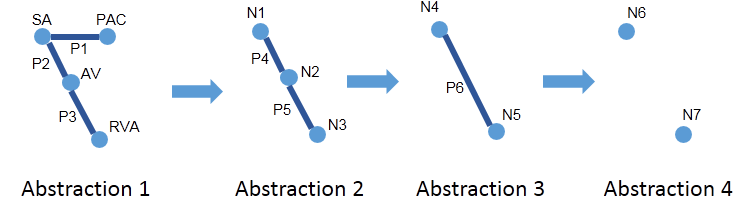
\includegraphics[width=0.9\textwidth]{figs/abs.png}
%%\vspace{-5pt}
%\caption{\small Heart Model Abstractions}
%%\vspace{-15pt}
%\label{fig:abs_exam}
%\end{figure}
